\documentclass
[
a4paper,															%Papierformat
11pt,																%Schriftgröße
twoside=true,														%Zweiseitig
openright,															%Neues Kapitel immer auf der rechten Seite
titlepage,															%Titelseite
headinclude,														%Seitengröße auch bei Kopfzeile
numbers=noenddot,													%Bei Kapiteln keine abschließenden Punkte
listof=numbered,													%Listingsverzeichnis
bibliography=totocnumbered,											%Literaturverzeichnis
]
{scrbook}															%Dokumenttyp
\usepackage[ngerman]{babel}											%Deutsch
\usepackage[bottom=1in,inner=1in,outer=20mm,top=20mm]{geometry}		%Ganze Seite
\usepackage{emptypage}												%Leere Seiten ohne Kopf und Fußzeile
\usepackage[headsepline]{scrlayer-scrpage}							%Kopf und Fußzeile
\pagestyle{scrheadings}												%Nummerierung in der Kopfzeile
\clearscrheadfoot													%Kopf und Fußzeile löschen
\rehead{\headmark}													%Kapitelname auf der geraden Seite innen
\ohead[\pagemark]{\pagemark}										%Seitennummerierung
\lohead{}															%Name auf der ungeraden Seite innen
\renewcommand*{\chapterpagestyle}{scrheadings}						%Kopf und Fußzeile auf Seiten mit Überschriften anders
\usepackage{graphicx}												%Bilder
\usepackage{caption}												%Tabellen Listings und Figuren mit beschriftung im Verzeichnissen
\usepackage[T1]{fontenc}											%Outputencoding
\usepackage{float}													%Plazierung von Floats (Bilder Tabellen)
\usepackage[utf8]{inputenc}											%UTF8
\usepackage{wrapfig}												%Textumfluss von Bildern, die nicht die ganze Seite Brauchen
\usepackage{setspace}												%Zeilenabstand
\usepackage{listings}												%Listings (=Code)
\usepackage{times}													%Schriftart Times Roman
\usepackage{courier}												%Schriftart Courier
\usepackage{multirow}												%Bessere Tabellenformatierung
\usepackage{array}													%Bessere Tabellenformatierung
\usepackage{xcolor}													%Farben für Codehighlighting oder ähnliches
\usepackage{appendix}												%Anhang Titelseite
\usepackage{tabularx}												%Bessere Tabellen
\usepackage{jurabib}												%Zitierung
\usepackage[bookmarks]{hyperref}									%Automatische Lesezeichen
\usepackage[printonlyused,withpage]{acronym}						%Für die Verwendung von Akronymen + Verzeichnis - printonlyused: Abkürzung nur im Verzeichnis wenn auch benutzt; withpage: Seite der 1. Verwendung im Verzeichnis anzeigen
\usepackage{dirtree}												%

\usepackage{titlesec}

\titleformat{\chapter}[display]
  {\bfseries\Large}
  {\filright\MakeUppercase{\chaptertitlename} \Huge\thechapter}
  {1ex}
  {\titlerule\vspace{1ex}\filleft}
  [\vspace{1ex}\titlerule]
\colorlet{punct}{red!60!black}
\colorlet{numb}{magenta!60!black}
\definecolor{background}{RGB}{255,255,255}
\definecolor{delim}{RGB}{20,105,176}
\definecolor{lightgreen}{HTML}{09885f}
\definecolor{green}{HTML}{008000}
\definecolor{red}{HTML}{a31515}    
\definecolor{editorGray}{rgb}{0.95, 0.95, 0.95}
\definecolor{htmlstrings}{HTML}{0000ff}
\definecolor{htmlattributes}{HTML}{ff0000}
\definecolor{htmltags}{HTML}{800000}
\definecolor{htmlcomments}{HTML}{008000}
\definecolor{C_net_comment}{rgb}{0.586,0.586,0.586}
\definecolor{C_net_keyword}{rgb}{0,0,0.898}
\definecolor{C_net_string}{rgb}{0.805,0.480,0}
\definecolor{C_net_preprocessor}{rgb}{0,0.597,0}

\lstdefinestyle{JavaStyle}{
  language=Java,
  columns=flexible,
  frame=single,
  frameround=tttt,
  showstringspaces=false,
  basicstyle=\footnotesize\ttfamily,
  literate=%
    {Ö}{{\"O}}1
    {Ä}{{\"A}}1
    {Ü}{{\"U}}1
    {ß}{{\ss}}1
    {ü}{{\"u}}1
    {ä}{{\"a}}1
    {ö}{{\"o}}1
    {~}{{\textasciitilde}}1
}

\lstdefinelanguage{json}{
    basicstyle=\footnotesize\ttfamily,
    showstringspaces=false,
    breaklines=true,
    frame=single,
    frameround=tttt,
    backgroundcolor=\color{background},
    literate=
     *{0}{{{\color{numb}0}}}{1}
      {1}{{{\color{numb}1}}}{1}
      {2}{{{\color{numb}2}}}{1}
      {3}{{{\color{numb}3}}}{1}
      {4}{{{\color{numb}4}}}{1}
      {5}{{{\color{numb}5}}}{1}
      {6}{{{\color{numb}6}}}{1}
      {7}{{{\color{numb}7}}}{1}
      {8}{{{\color{numb}8}}}{1}
      {9}{{{\color{numb}9}}}{1}
      {:}{{{\color{punct}{:}}}}{1}
      {,}{{{\color{punct}{,}}}}{1}
      {\{}{{{\color{delim}{\{}}}}{1}
      {\}}{{{\color{delim}{\}}}}}{1}
      {[}{{{\color{delim}{[}}}}{1}
      {]}{{{\color{delim}{]}}}}{1},
}

\lstdefinelanguage{Typescript}{
  keywords={typeof, new, true, false, catch, function, return, null, catch, switch, var, if, for, in, while, do, else, case, break, class, export, boolean, throw, implements, import, this, constructor, from, =>, public, private, string, new},
  keywordstyle=\color{blue},
  identifierstyle=\color{black},
  sensitive=false,
  comment=[l]{//},
  morecomment=[s]{/*}{*/},
  commentstyle=\color{green}\ttfamily,
  stringstyle=\color{red}\ttfamily,
  morestring=[b]',
  morestring=[b]"
}

\lstdefinestyle{TypescriptStyle}{
   language=Typescript,
   backgroundcolor=\color{white},
   extendedchars=true,
   basicstyle=\footnotesize\ttfamily,
   showstringspaces=false,
   showspaces=false,
   numbers=left,
   numberstyle=\footnotesize,
   numbersep=9pt,
   tabsize=2,
   breaklines=true,
   showtabs=false,
   captionpos=b,
   literate={ä}{{\"a}}1 {ö}{{\"o}}1 {ü}{{\"u}}1
   {0}{{{\ProcessDigit{0}}}}1
   {1}{{{\ProcessDigit{1}}}}1
   {2}{{{\ProcessDigit{2}}}}1
   {3}{{{\ProcessDigit{3}}}}1
   {4}{{{\ProcessDigit{4}}}}1
   {5}{{{\ProcessDigit{5}}}}1
   {6}{{{\ProcessDigit{6}}}}1
   {7}{{{\ProcessDigit{7}}}}1
   {8}{{{\ProcessDigit{8}}}}1
   {9}{{{\ProcessDigit{9}}}}1
   {<=}{{\(\leq\)}}1,
   morestring=[b]",
   morestring=[b]',
   morecomment=[l]//,
}


\lstdefinelanguage{CSS}{
   keywords={accelerator,azimuth,background,background-attachment,
            background-color,background-image,background-position,
            background-position-x,background-position-y,background-repeat,
            behavior,border,border-bottom,border-bottom-color,
            border-bottom-style,border-bottom-width,border-collapse,
            border-color,border-left,border-left-color,border-left-style,
            border-left-width,border-right,border-right-color,
            border-right-style,border-right-width,border-spacing,
            border-style,border-top,border-top-color,border-top-style,
            border-top-width,border-width,bottom,caption-side,clear,
            clip,color,content,counter-increment,counter-reset,cue,
            cue-after,cue-before,cursor,direction,display,elevation,
            empty-cells,filter,float,font,font-family,font-size,
            font-size-adjust,font-stretch,font-style,font-variant,
            font-weight,height,ime-mode,include-source,
            layer-background-color,layer-background-image,layout-flow,
            layout-grid,layout-grid-char,layout-grid-char-spacing,
            layout-grid-line,layout-grid-mode,layout-grid-type,left,
            letter-spacing,line-break,line-height,list-style,
            list-style-image,list-style-position,list-style-type,margin,
            margin-bottom,margin-left,margin-right,margin-top,
            marker-offset,marks,max-height,max-width,min-height,
            min-width,-moz-binding,-moz-border-radius,
            -moz-border-radius-topleft,-moz-border-radius-topright,
            -moz-border-radius-bottomright,-moz-border-radius-bottomleft,
            -moz-border-top-colors,-moz-border-right-colors,
            -moz-border-bottom-colors,-moz-border-left-colors,-moz-opacity,
            -moz-outline,-moz-outline-color,-moz-outline-style,
            -moz-outline-width,-moz-user-focus,-moz-user-input,
            -moz-user-modify,-moz-user-select,orphans,outline,
            outline-color,outline-style,outline-width,overflow,
            overflow-X,overflow-Y,padding,padding-bottom,padding-left,
            padding-right,padding-top,page,page-break-after,
            page-break-before,page-break-inside,pause,pause-after,
            pause-before,pitch,pitch-range,play-during,position,quotes,
            -replace,richness,right,ruby-align,ruby-overhang,
            ruby-position,-set-link-source,size,speak,speak-header,
            speak-numeral,speak-punctuation,speech-rate,stress,
            scrollbar-arrow-color,scrollbar-base-color,
            scrollbar-dark-shadow-color,scrollbar-face-color,
            scrollbar-highlight-color,scrollbar-shadow-color,
            scrollbar-3d-light-color,scrollbar-track-color,table-layout,
            text-align,text-align-last,text-decoration,text-indent,
            text-justify,text-overflow,text-shadow,text-transform,
            text-autospace,text-kashida-space,text-underline-position,top,
            unicode-bidi,-use-link-source,vertical-align,visibility,
            voice-family,volume,white-space,widows,width,word-break,
            word-spacing,word-wrap,writing-mode,z-index,zoom},  
  sensitive=true,
  morecomment=[l]{//},
  morecomment=[s]{/*}{*/},
  morestring=[b]',
  morestring=[b]",
  alsoletter={:},
  alsodigit={-}
}
\lstdefinelanguage{HTML5}{
  language=html,
  sensitive=true, 
  alsoletter={<>=-},
  otherkeywords={
            % HTML tags
            <, </, >,
            </a, <a, </a>,
            </abbr, <abbr, </abbr>,
            </address, <address, </address>,
            </area, <area, </area>,
            </area, <area, </area>,
            </article, <article, </article>,
            </aside, <aside, </aside>,
            </audio, <audio, </audio>,
            </audio, <audio, </audio>,
            </b, <b, </b>,
            </base, <base, </base>,
            </bdi, <bdi, </bdi>,
            </bdo, <bdo, </bdo>,
            </blockquote, <blockquote, </blockquote>,
            </body, <body, </body>,
            </br, <br, </br>,
            </button, <button, </button>,
            </canvas, <canvas, </canvas>,
            </caption, <caption, </caption>,
            </cite, <cite, </cite>,
            </code, <code, </code>,
            </col, <col, </col>,
            </colgroup, <colgroup, </colgroup>,
            </data, <data, </data>,
            </datalist, <datalist, </datalist>,
            </dd, <dd, </dd>,
            </del, <del, </del>,
            </details, <details, </details>,
            </dfn, <dfn, </dfn>,
            </div, <div, </div>,
            </dl, <dl, </dl>,
            </dt, <dt, </dt>,
            </em, <em, </em>,
            </embed, <embed, </embed>,
            </fieldset, <fieldset, </fieldset>,
            </figcaption, <figcaption, </figcaption>,
            </figure, <figure, </figure>,
            </footer, <footer, </footer>,
            </form, <form, </form>,
            </h1, <h1, </h1>,
            </h2, <h2, </h2>,
            </h3, <h3, </h3>,
            </h4, <h4, </h4>,
            </h5, <h5, </h5>,
            </h6, <h6, </h6>,
            </head, <head, </head>,
            </header, <header, </header>,
            </hr, <hr, </hr>,
            </html, <html, </html>,
            </i, <i, </i>,
            </iframe, <iframe, </iframe>,
            </img, <img, </img>,
            </input, <input, </input>,
            </ins, <ins, </ins>,
            </kbd, <kbd, </kbd>,
            </keygen, <keygen, </keygen>,
            </label, <label, </label>,
            </legend, <legend, </legend>,
            </li, <li, </li>,
            </link, <link, </link>,
            </main, <main, </main>,
            </map, <map, </map>,
            </mark, <mark, </mark>,
            </math, <math, </math>,
            </menu, <menu, </menu>,
            </menuitem, <menuitem, </menuitem>,
            </meta, <meta, </meta>,
            </meter, <meter, </meter>,
            </nav, <nav, </nav>,
            </noscript, <noscript, </noscript>,
            </object, <object, </object>,
            </ol, <ol, </ol>,
            </optgroup, <optgroup, </optgroup>,
            </option, <option, </option>,
            </output, <output, </output>,
            </p, <p, </p>,
            </param, <param, </param>,
            </pre, <pre, </pre>,
            </progress, <progress, </progress>,
            </q, <q, </q>,
            </rp, <rp, </rp>,
            </rt, <rt, </rt>,
            </ruby, <ruby, </ruby>,
            </s, <s, </s>,
            </samp, <samp, </samp>,
            </script, <script, </script>,
            </section, <section, </section>,
            </select, <select, </select>,
            </small, <small, </small>,
            </source, <source, </source>,
            </span, <span, </span>,
            </strong, <strong, </strong>,
            </style, <style, </style>,
            </summary, <summary, </summary>,
            </sup, <sup, </sup>,
            </svg, <svg, </svg>,
            </table, <table, </table>,
            </tbody, <tbody, </tbody>,
            </td, <td, </td>,
            </template, <template, </template>,
            </textarea, <textarea, </textarea>,
            </tfoot, <tfoot, </tfoot>,
            </th, <th, </th>,
            </thead, <thead, </thead>,
            </time, <time, </time>,
            </title, <title, </title>,
            </tr, <tr, </tr>,
            </track, <track, </track>,
            </u, <u, </u>,
            </ul, <ul, </ul>,
            </var, <var, </var>,
            </video, <video, </video>,
            </wbr, <wbr, </wbr>,
            </ng-template, <ng-template, </ng-template>,
            </ng-container, <ng-container, </ng-container>,
            </router-outlet, <router-outlet, </router-outlet>,
            </app-cat, <app-cat, </app-cat>,
            </app-login, <app-login, </app-login>,
            />, <!
            },  
            ndkeywords={
            % General
            =,
            % HTML attributes
            accept=, accept-charset=, accesskey=, action=, align=, alt=, async=, autocomplete=, autofocus=, autoplay=, autosave=, bgcolor=, border=, buffered=, challenge=, charset=, checked=, cite=, class=, code=, codebase=, color=, cols=, colspan=, content=, contenteditable=, contextmenu=, controls=, coords=, data=, datetime=, default=, defer=, dir=, dirname=, disabled=, download=, draggable=, dropzone=, enctype=, for=, form=, formaction=, headers=, height=, hidden=, high=, href=, hreflang=, http-equiv=, icon=, id=, ismap=, itemprop=, keytype=, kind=, label=, lang=, language=, list=, loop=, low=, manifest=, max=, maxlength=, media=, method=, min=, multiple=, name=, novalidate=, open=, optimum=, pattern=, ping=, placeholder=, poster=, preload=, pubdate=, radiogroup=, readonly=, rel=, required=, reversed=, rows=, rowspan=, sandbox=, scope=, scoped=, seamless=, selected=, shape=, size=, sizes=, span=, spellcheck=, src=, srcdoc=, srclang=, start=, step=, style=, summary=, tabindex=, target=, title=, type=, usemap=, value=, width=, wrap=, click, ngClass, hidden, ngbDropdown, ngbDropdownToggle, ngbDropdownMenu, ngFor=, ngIf=, i18n, required, ngModel, placement=, ngSubmit, disabled, minlength=, maxlength=, keyup, change, class.input-error, @SaveAnimation, routerLink=,
            % CSS properties
            accelerator:,azimuth:,background:,background-attachment:,
            background-color:,background-image:,background-position:,
            background-position-x:,background-position-y:,background-repeat:,
            behavior:,border:,border-bottom:,border-bottom-color:,
            border-bottom-style:,border-bottom-width:,border-collapse:,
            border-color:,border-left:,border-left-color:,border-left-style:,
            border-left-width:,border-right:,border-right-color:,
            border-right-style:,border-right-width:,border-spacing:,
            border-style:,border-top:,border-top-color:,border-top-style:,
            border-top-width:,border-width:,bottom:,caption-side:,clear:,
            clip:,color:,content:,counter-increment:,counter-reset:,cue:,
            cue-after:,cue-before:,cursor:,direction:,display:,elevation:,
            empty-cells:,filter:,float:,font:,font-family:,font-size:,
            font-size-adjust:,font-stretch:,font-style:,font-variant:,
            font-weight:,height:,ime-mode:,include-source:,
            layer-background-color:,layer-background-image:,layout-flow:,
            layout-grid:,layout-grid-char:,layout-grid-char-spacing:,
            layout-grid-line:,layout-grid-mode:,layout-grid-type:,left:,
            letter-spacing:,line-break:,line-height:,list-style:,
            list-style-image:,list-style-position:,list-style-type:,margin:,
            margin-bottom:,margin-left:,margin-right:,margin-top:,
            marker-offset:,marks:,max-height:,max-width:,min-height:,
            min-width:,transition-duration:,transition-property:,
            transition-timing-function:,transform:,
            -moz-transform:,-moz-binding:,-moz-border-radius:,
            -moz-border-radius-topleft:,-moz-border-radius-topright:,
            -moz-border-radius-bottomright:,-moz-border-radius-bottomleft:,
            -moz-border-top-colors:,-moz-border-right-colors:,
            -moz-border-bottom-colors:,-moz-border-left-colors:,-moz-opacity:,
            -moz-outline:,-moz-outline-color:,-moz-outline-style:,
            -moz-outline-width:,-moz-user-focus:,-moz-user-input:,
            -moz-user-modify:,-moz-user-select:,orphans:,outline:,
            outline-color:,outline-style:,outline-width:,overflow:,
            overflow-X:,overflow-Y:,padding:,padding-bottom:,padding-left:,
            padding-right:,padding-top:,page:,page-break-after:,
            page-break-before:,page-break-inside:,pause:,pause-after:,
            pause-before:,pitch:,pitch-range:,play-during:,position:,quotes:,
            -replace:,richness:,right:,ruby-align:,ruby-overhang:,
            ruby-position:,-set-link-source:,size:,speak:,speak-header:,
            speak-numeral:,speak-punctuation:,speech-rate:,stress:,
            scrollbar-arrow-color:,scrollbar-base-color:,
            scrollbar-dark-shadow-color:,scrollbar-face-color:,
            scrollbar-highlight-color:,scrollbar-shadow-color:,
            scrollbar-3d-light-color:,scrollbar-track-color:,table-layout:,
            text-align:,text-align-last:,text-decoration:,text-indent:,
            text-justify:,text-overflow:,text-shadow:,text-transform:,
            text-autospace:,text-kashida-space:,text-underline-position:,top:,
            unicode-bidi:,-use-link-source:,vertical-align:,visibility:,
            voice-family:,volume:,white-space:,widows:,width:,word-break:,
            word-spacing:,word-wrap:,writing-mode:,z-index:,zoom:
            },  
  morecomment=[s]{<!--}{-->},
  tag=[s]
}

\lstdefinestyle{HtmlStyle}{%
	% Basic design
 	backgroundcolor=\color{editorGray},
 	basicstyle={\small\ttfamily},
    numbers=left,
    stepnumber=1,
    firstnumber=1,
    numberfirstline=true,
    % Code design   
    keywordstyle=\color{blue}\bfseries,
    commentstyle=\color{darkgray}\ttfamily,
    ndkeywordstyle=\color{editorGreen}\bfseries,
    stringstyle=\color{editorOcher},
    % Code
    language=HTML5,
    alsodigit={.:;},
    tabsize=2,
    showtabs=false,
    showspaces=false,
    showstringspaces=false,
    extendedchars=true,
    breaklines=true,
	literate={ä}{{\"a}}1 {ö}{{\"o}}1 {ü}{{\"u}}1 {ß}{{\ss}}1,        
    }

\newcommand\digitstyle{\color{lightgreen}}
\makeatletter
\newcommand{\ProcessDigit}[1]
{%
  \ifnum\lst@mode=\lst@Pmode\relax%
   {\digitstyle #1}%
  \else
    #1%
  \fi
}
\makeatother

\setlength{\parindent}{0em}
 
\subject{
\includegraphics[scale=0.7]{Bilder/Logo}}
\title{Katzenfütterungsanlage}
\subtitle{HTBLA Kaindorf an der Sulm\\Grazer Straße 202, A-8430 Kaindorf an der Sulm\\Ausbildungsschwerpunkt Mechatronik und Automatisierungstechnik}
\author{Florian Greistorfer, Florian Harrer, Dominik Pichler, Julian Wolf}
\date{Abgabedatum: 05.04.2018}
\publishers{Betreut von:\\Dipl.-Ing. Manfred Steiner\\Dipl.Ing. Dr. Gerhard Pretterhofer\\Otto}
\begin{document}
\onehalfspace
\maketitle
\setcounter{tocdepth}{5}
\setcounter{secnumdepth}{4}

\tableofcontents
\mainmatter
\lohead{Florian Greistorfer}
\chapter{Webserver und Client}

\section{Begriffserklärungen}

\subsection{Server}
Ein Programm, der oder das Zugriff auf eine Resource oder einen Dienst in einem Netzwerk ermöglicht

\subsection{Client}
Ein Programm, der oder das auf einen Server zugreift

\section{Anforderungen}

\subsection{Webserver}
Auf der Katzenfütterungsanlage läuft ein Webserver, der es ermöglicht, dass der Benutzer das Gerät über das Internet erreichen kann. Hauptaufgaben des Servers sind dabei, Daten bereitzustellen, zu verabeiten und zu speichern und den Webclient zur Verfügung zu stellen.

\subsection{Client}
Der Client soll dem Benutzer ermöglichen, die Katzenfütterungsanlage über einen Webbrowser zu steuern. Ein Benutzername und ein Passwort sind erforderlich, damit man das Gerät bedienen kann. Das Design soll eindeutig und übersichtlich gehalten sein. Auf der Startseite sollen die eingestellten Fütterungszeiten zu sehen sein und eine allgemeine Übersicht. Über eine Navigationsleiste sollen die weiteren Seiten erreichbar sein:

\begin{itemize}
\item[•]Fütterrungszeiten
\item[•]Positionsinfo
\item[•]Geräteinfo
\item[•]Update
\end{itemize}

\section{Voruntersuchung}

\subsection{HTTP/HTTPS}
Das \ac{HTTP} ist der Kommunikationsstandart auf dem das Internet basiert. Eine HTTP Session wird über eine Anfrage über das \ac{TCP} an einen Server auf den Port 80 initiiert. Der Server, der auf diesem Port auf eine Anfrage wartet sendet eine Statusmeldung wie z.B. \inlinecode{bash}{HTTP/1.1 200 OK} und eine eigene Nachricht zurück. Diese Nachricht ist meist die angeforderte Resource oder eine Fehlermeldung. \ac{HTTPS} ist die Verschlüsselte Version von \ac{HTTP}. Die meist gebrauchten Anfragen sind:

\begin{itemize}
\item[•] \textbf{GET}: Fordert eine Representation der Resource an. Ein GET Request darf nur Daten abfragen und darf keinen anderen Einfluss haben.
\item[•] \textbf{PUT}: Fordert das speicher der Daten, die sich im Request-Body befinden, an. Wenn bereits eine Resource an der angegebenen \ac{URI} existiert, so wird diese geupdatet, sonst wir die Resource erstellt.
\item[•] \textbf{POST}: Fordert das speichern der Daten, die sich im Request-Body befinden, unter der angegebenen \ac{URI} an. 
\item[•] \textbf{DELETE}: Fordert das Löschen der Resource unter der angegebenen \ac{URI} an.
\end{itemize}

\subsection{JavaScript}
JavaScript ist die Sprache des Internets. Jeder herkömmliche Browser ist in der Lage, JavaScript auszuführen. Mit JavaScript ist es möglich, das Aussehen einer Webseite während der Laufzeit zu ändern, Dinge zu entfernen, hinzufügen und animieren. JavaScript ist eine objektorientierte Sprache. Es hebt sich von anderen Sprachen vorallem dadurch ab, dass die Datentypen von Variable nicht fix sind. Das bedeutet, wenn eine Variable den Datentyp \textit{number} hat und es wird ein String angehängt, verändert sich der Datentyp automatisch auf \textit{string}.

\subsection{Node.js}
Node.js ist eine Laufzeitumgebung, die es ermöglicht, dass Javascript direkt auf einem Rechner ausgeführt werden kann. Node.js kommt mit dem \ac{npm}. Mithilfe diesem Tools ist es möglich, Module zu installieren, updaten, löschen und veröffentlichen. Diese Module werden im Ordner \textit{/node\_modules} installiert und in der Datei \textit{package.json} unter \textit{dependencies}, oder mit der option \inlinecode{bash}{--save-dev} unter \textit{dev-dependencies} eingetragen. Ein neues Projekt erstellt man mit \inlinecode{bash}{npm init}. Dieses Tool erstellt die Datei \textit{package.json}, in der alle Abhängigkeiten und Informationen über das Projekt stehen. Wenn man ein Projekt kopiert, braucht man den \textit{/node\_modules} Ordner nicht mit kopieren. Man muss nur im Zielordner einmal \inlinecode{bash}{npm install} aufrufen.

\subsection{TypeScript}
TypeScript ist eine, von Microsoft entwickelte, Weiterentwicklung von JavaScript. Das bedeutet, jeder gültige JavaScript Code ist auch ein gültiger TypeScript Code. TypeScript wird vom TypeScript Compiler in sauberes JavaScript übersetzt. TypeScript ist sehr gut für größere Anwendungen geeignet. Typescript hat strenge Datentypen, Klassen und Vererbung. Die Datentypen von TypeScript sind:

\begin{itemize}
\item[•] \textbf{String}: eine Unicode codierte Zeichenkette
\item[•] \textbf{Number}: eine vorzeichenbehaftete Gleitkommazahl, kann auch hexadezimal, octal oder binär sein
\item[•] \textbf{Boolean}: true oder false
\item[•] \textbf{Array}: eine Liste von Elementen des gleichen Datentyps
\item[•] \textbf{Tuple}: eine Liste von Elementen unterschiedlichen Datentyps deren Anzahl bekannt ist
\item[•] \textbf{Enum}: eine Möglichkeit, numerischen Werten Namen zu geben
\item[•] \textbf{Any}: Datentyp unbekannt, wird behandelt wie in JavaScript
\item[•] \textbf{Void}: kein Datentyp, meist Rückgabewert bei Funktionen
\item[•] \textbf{Null}: leerer Wert, kann allen anderen zugewiesen werden
\item[•] \textbf{Undefined}: kein Wert, kann allen anderen zugewiesen werden
\item[•] \textbf{Never}: wenn ein Wert niemals auftreten kann z.B. eine Funktion die immer einen Fehler produziert
\end{itemize}

Damit JavaScript Module von TypeScript verwendet werden können, benötigen sie sogenannte Type Annotations. Diese können bei den meisten bekannteren Modulen über den \ac{npm} installiert werden. Diese Pakete haben den Namenspräfix \textit{@types/}, das bedeutet, dass zum Beispiel die Type Annotations des Express Moduls über \inlinecode{bash}{npm install --save-dev @types/express} installiert werden können. Sollten keine Type Annotations für ein Modul vorhanden sein, muss man diese selbst erstellen.

\subsection{express}
Express ist ein Javascript Modul, dass auf dem Node.js Modul \textit{http} bzw \textit{https} aufbaut. In diesen Modulen ist bereits alles enthalten, dass benötigt wird, um einen Webserver zu programmieren. Express nimmt uns die meiste Arbeit ab und bietet viele weitere Möglichkeiten.

\subsection{JSON}
\ac{JSON} ist die Textrepresentation eines JavaScript Objekts. Die möglichen Datentypen sind:

\begin{itemize}
\item[•] \textbf{string}: 0 oder mehrere unicode Zeichen innerhalb Doppelhochkommas
\item[•] \textbf{boolean}: true oder false
\item[•] \textbf{number}: Eine vorzeichenbehaftete Zahl, die auch die E Notation unterstützt z.B. 0.2E4 (=2000)
\item[•] \textbf{Array}: Eine geordnete Liste von 0 oder mehreren Werten innerhalb viereckigen Klammern, Elemente sind getrennt durch Kommas.
\item[•] \textbf{Object}: Eine ungeordnete Sammlung von Name-Wert-Paaren, wo die Namen, die auch Keys genannt werden, Strings sind; Jeder Key sollte eindeutig sein; Innerhalb geschwungener Klammern; Paare sind durch Komma getrennt
\item[•] \textbf{null}: Ein leerer Wert
\end{itemize}

\begin{lstlisting}[style=JSON,caption=\ac{JSON} Beispiel]
{
	"Object": {	
		"string": "name",
		"number": 10E5,
		"boolean": true,
		"Array": [
			{
				"string": "wert",
				"number": 1
			},
			{
				"string": "wert",
				"number": 2
			}
		]
	}
}
\end{lstlisting}

\subsection{JSON Web Token}
\ac{JWT} ist ein JSON-basierter, offener Standart für das erstellen von Access Tokens. Mithilfe eines \ac{JWT} kann ein Client sich ausweisen. Ein \ac{JWT} wird vom Server entweder mit einem Secret oder seinem privaten Schlüssel signiert. Dadurch können Server und Client beide überprüfen, ob der Token legitim ist. Ein \ac{JWT} besteht aus drei Teilen. Dem Header, der Payload und der Signature. Im Header steht der fürs Verschlüsseln der Signatur benutzte Algorythmus z.B: \inlinecode{JSON}{\{"alg":"RS256","typ":"JWT"\}}. Im Payload stehen die Daten, die entweder den Client ausweisen oder ähnliche Information. Beispiel: \inlinecode{JSON}{\{"user": "cat", "iat": 1520875121, "exp": 1520911121\}} \textit{iat} bedeutet \textit{issued at} und sagt aus, wann der Token generiert wurde. In der Signature steht der Key, der unsignierte Token, das ist der Header und die Payload Base64 codiert, und die Signatur. Alle drei Teile werden Base64 codiert und mittels Punkt voneinander getrennt.

\subsection{MongoDB}
MongoDB ist eine schemenlose Datenbank. Schemenlos bedeutet, dass die Datenbank, im vergleich zu schemenbehafteten Datenbanken, keine klare Strukturierung benötigt. Einer schemenlosen Datenbank kann man einfach Daten geben und wieder abfragen. Eine schemenbehaftete Datenbank ist in Zeilen und Spalten unterteilt. Diese müssen vorher feststehen. Da Raspian, das Betriebssystem vom Raspberry Pi, nur 32 Bit ist und MongoDB ab Version 3 nur mehr in 64 Bit erhältlich ist, mussten wir auf eine ältere Version wechseln. Die Verbindung der MongoDB Datenbank erfolgt über einen Driver. Der Driver muss mit der Datenbankversion übereinstimmen. MongoDB ist ein \ac{DBS}, das bedeutet, ein Server läuft auf dem Port 27017, über den alle Datenbanken im System erreichbar sind z.B. die Datenbank \textit{fuettr} ist über \inlinecode{bash}{localhost:27017/fuettr} erreichbar. Eine Gruppe von Daten nennt man Collection. Zugriff auf die Datenbank erfolgt serverseitig wie folgt:

\begin{lstlisting}[caption=Verbinden mit dem \ac{DBS},style=TS]
const dbServer = await mongodb.MongoClient.connect(url);
\end{lstlisting}

\begin{lstlisting}[caption=Auswählen der Datenbank,style=TS]
const dbFuettr = await dbServer.db('fuettr');
\end{lstlisting}

\begin{lstlisting}[caption=Auswählen der Collection,style=TS]
const collTimes = await dbFuettr.collection('data_times');
\end{lstlisting}

\begin{lstlisting}[caption=Auslesen aller Datensätze mit einem Identifier,style=TS]
const Times = await this._times.find({ identifier: 'Times' }).toArray();
\end{lstlisting}

\begin{lstlisting}[caption=Überschreiben eines Datensatzes mit einem Identifier,style=TS]
this._times.updateOne({ identifier: 'Times' }, { $set: times });
\end{lstlisting}

\subsection{Angular 2/4}
Angular ist ein TypeScript Framework, das aus dem Javascript-Framework AngularJS weiterentwickelt wurde. Es wird von Google entwickelt. Angular ist gegliedert in Module. Die grobe Struktur wird in der Abbildung \ref{Angular Struktur} dargestellt.

\begin{figure}[H]
      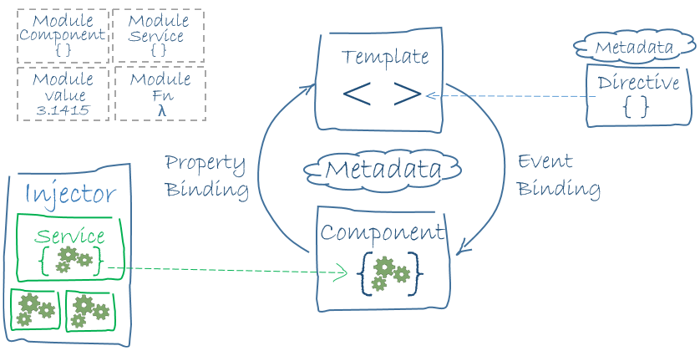
\includegraphics[width=1\textwidth]{Bilder/Greistorfer/Angular}
      \caption{Angular Struktur}
      \label{Angular Struktur}
\end{figure}

\subsubsection{Modules}
Jede Angular App ist in \textit{Module}s gegliedert. \textit{Module}s fassen meist ähnliche Funktionen zusammen. Jede App muss mindestens ein \textit{Module} enthalten. Dies heißt standartmäßig \textit{AppModule}. Ein \textit{Module} ist die größte Einheit einer Angular App.  Ein \textit{Module} kann folgende Komponenten beinhalten:

\begin{itemize}
\item[•]Services
\item[•]Andere Module
\item[•]View Classes
\begin{itemize}
\item[-]Components
\item[-]Directives
\item[-]Pipes
\end{itemize}
\end{itemize}

\subsubsection{Libraries}
Eine Angular Library ist ein Modul, das \textit{decorator} und \textit{Modules} exportiert. Diese können von \textit{Components} und \textit{Modules} importiert werden. Der Name jeder Angular library beginnt mit \textit{@angular}. Angular libraries können mit dem \ac{npm} installiert werden.

\subsubsection{Components}
Ein \textit{Component} kontrolliert einen Teil des Bildschirms, den sogenannten \textit{view}. Die Logik des \textit{Component}s wird in einer Klasse definiert. Die Klasse interagiert mit dem \textit{view} durch eine \ac{API} von Eigenschaften und Methoden.

\subsubsection{Templates}
Das Aussehen des \textit{view}s wird in einem \textit{Template} definiert. Ein \textit{Template} ist eine \ac{HTML} Datei, mit Angular's Template Syntax. Das bedeutet, dass einige Zusatzbefehle vorkommen können. Beispiele hierfür sind:

\begin{itemize}
\item[•]*ngFor
\item[•]*ngIf
\item[•]\{\{variable\}\}
\item[•](click)
\item[•][variable]
\item[•]<app-route>
\end{itemize}

\subsubsection{Data binding}
\begin{wrapfigure}{l}{0.5\textwidth}
\vspace{-30pt}
  \begin{center}
    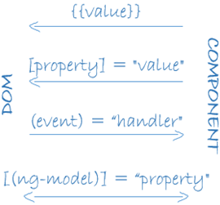
\includegraphics[width=0.5\textwidth]{Bilder/Greistorfer/databinding}
  \end{center}
  \caption{Angular Databinding}
  \label{Angular Databinding}
  \vspace{-10pt}
\end{wrapfigure}



\subsubsection{Services}

\subsection{Bootstrap}
Bootstrap ist eine CSS Bibliothek, die die Möglichkeit bietet, bereits vorgefertigte Komponenten auf unserer Website zu verwenden. An erster Stelle stehen bei Bootstrap responsive Design und Mobilgeräte. Responsive bedeutet, dass die Elemente sich an die breite des Bildschirms anpassen. Dadurch erspart man sich als nicht sehr designaffiner Programmierer viel Arbeit. Auf der offiziellen Bootstrap Website kann man außerdem verschiedene Themes auswählen. Bootstrap wurde von Twitter entwickelt und ist entweder über den \ac{npm} oder über Bootstraps eigenes \ac{CDN} erhältlich.

\section{Umsetzung}

\subsection{Projektstruktur}
\dirtree{%
.1 Webserver.
.2 server.
.3 dist.
.3 keys.
.3 node\_modules.
.3 public.
.3 src.
.4 views.
.2 ngx.
.3 dist.
.3 e2e.
.3 node\_modules.
.3 src.
.4 app.
.5 components.
.5 services.
.4 assets.
.4 environments.
.4 i18n.
}


\subsection{Client}

\subsubsection{Design}
Das Design sollte übersichtlich und einfach gestaltet werden. Der Benutzer soll auf den ersten Blick die wichtigsten Funktionen und Informationen erkennen können. \\

\begin{wrapfigure}{r}{0.7\textwidth}
\vspace{-30pt}
  \begin{center}
    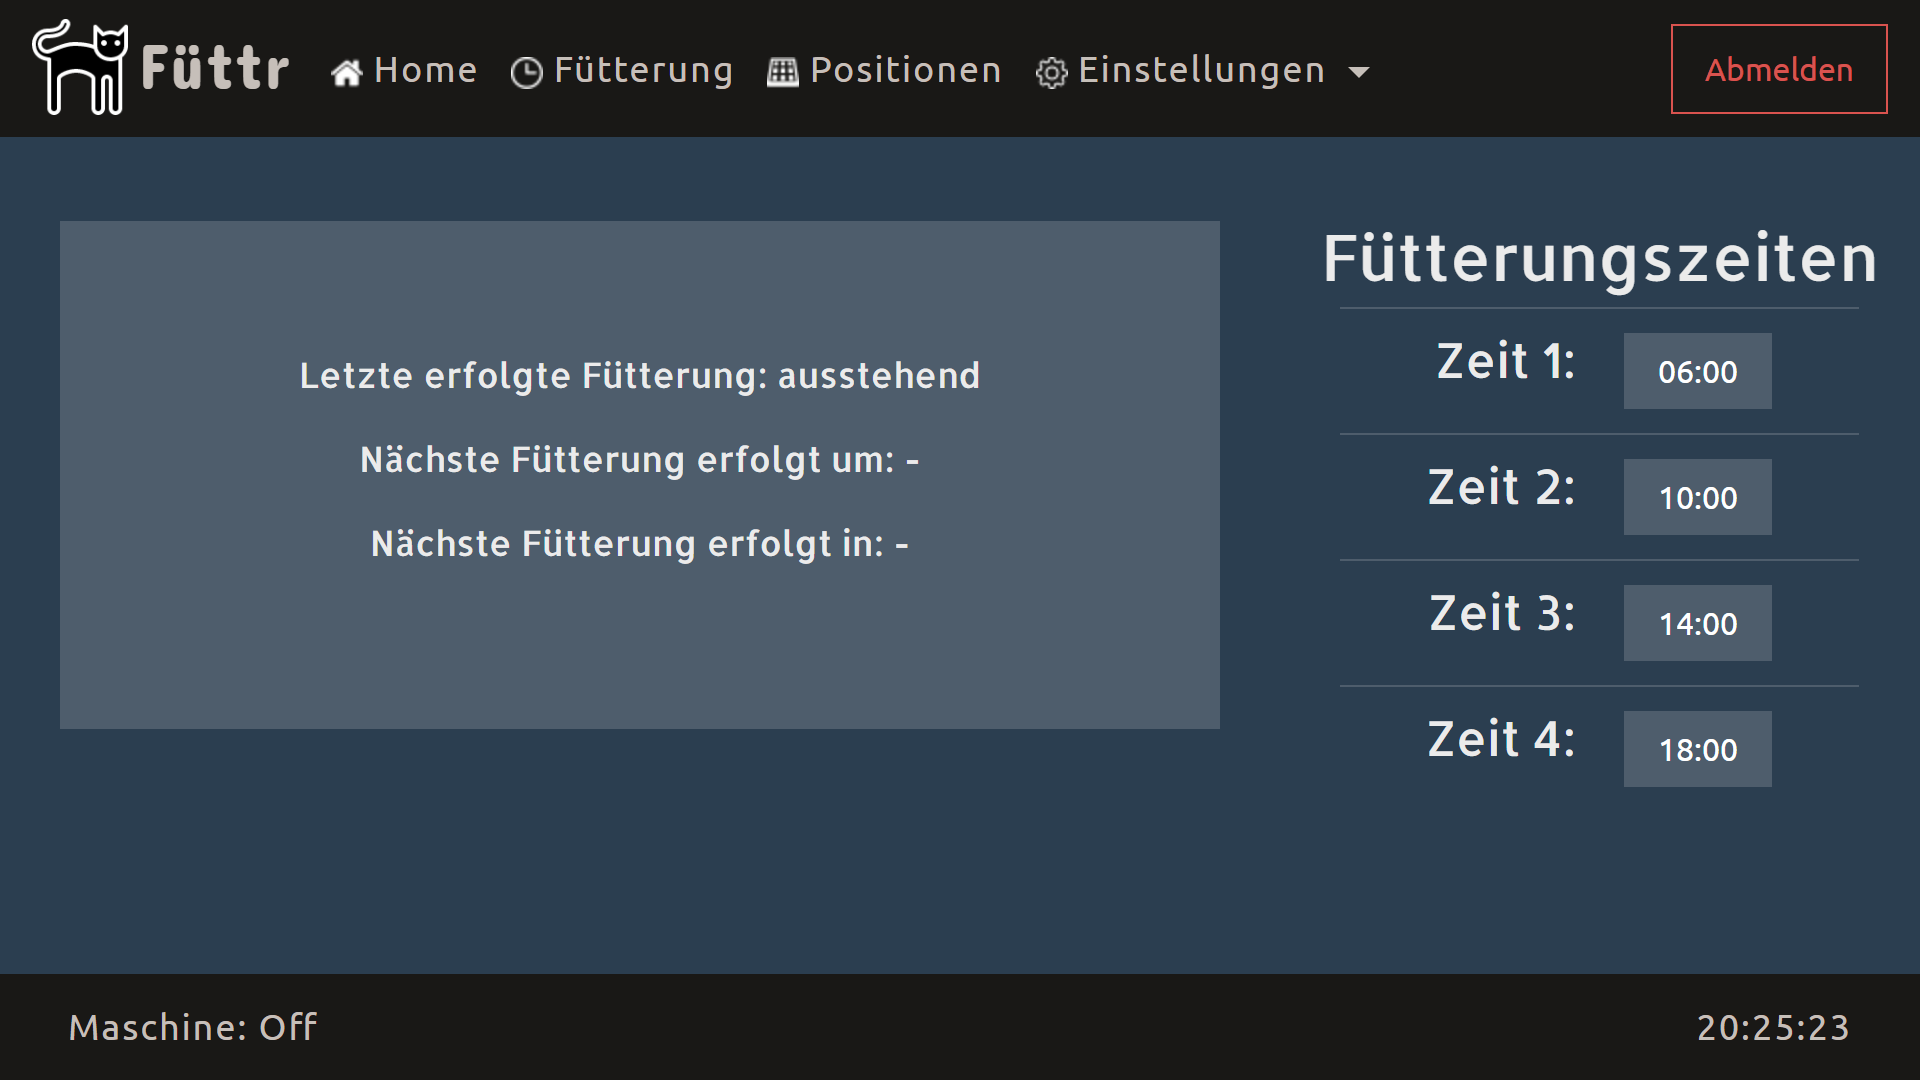
\includegraphics[width=0.7\textwidth]{Bilder/Greistorfer/Home}
  \end{center}
  \caption{Startseite}
  \label{Startseite}
  \vspace{-10pt}
\end{wrapfigure}

Auf der Starseite sind alle wichtigen Informationen übersichtlich dargestellt. Auf der linken Seite werden die Uhrzeit der letzten erfolgreichen Fütterung, die Zeit der nächsten Fütterung und die Zeit bis zur nächsten Fütterung dargestellt. Darunter werden Fehler und Warnungen, fals welche auftreten sollten, angezeigt. Da unbekannt ist, wie viele Fehler und Warnungen auftreten, werden diese in einem *ngFor aufgelistet. Auf der rechten Seite sind die aktiven Fütterungszeiten aufgelistet. \\

\begin{wrapfigure}{r}{0.7\textwidth}
\vspace{-30pt}
  \begin{center}
    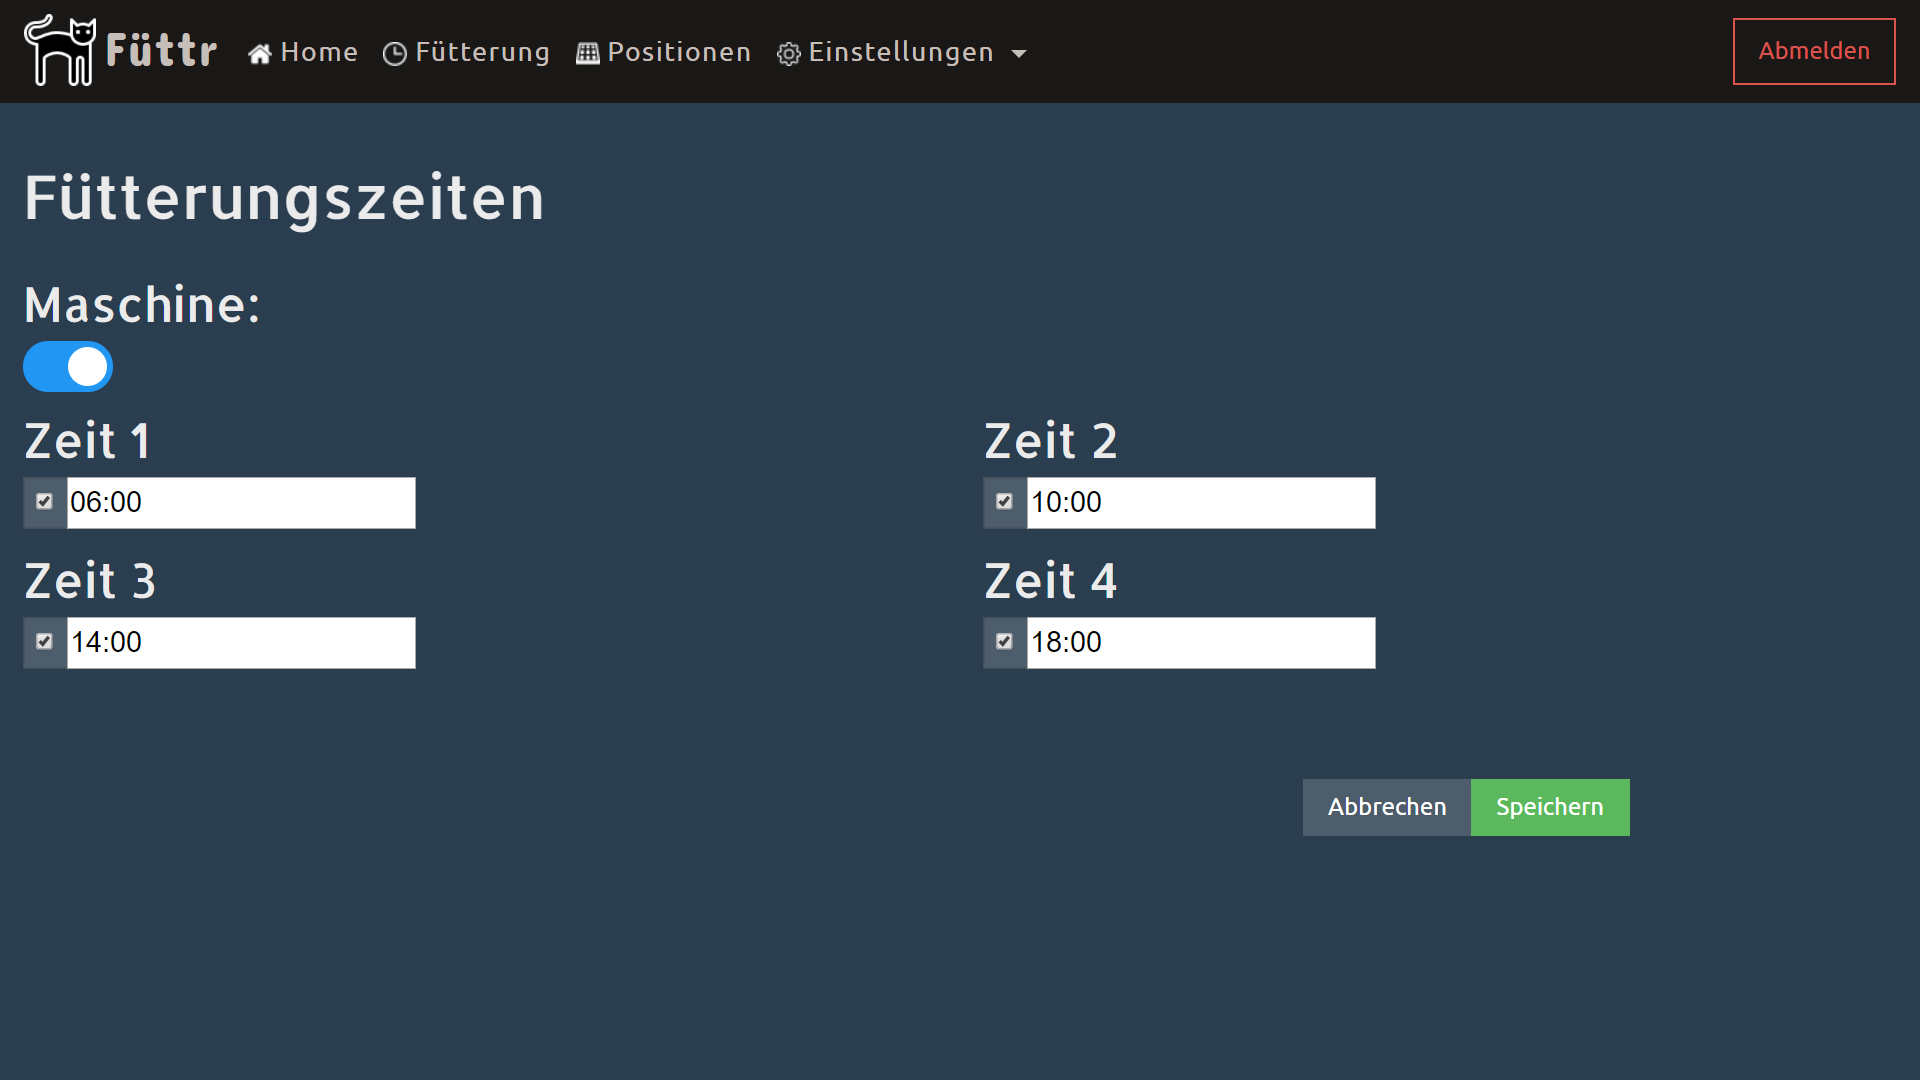
\includegraphics[width=0.7\textwidth]{Bilder/Greistorfer/Fuetterungszeiten}
  \end{center}
  \caption{Fütterungszeiten}
  \label{Fütterungszeiten}
  \vspace{-10pt}
\end{wrapfigure}

Auf der Fütterungszeiten-Seite kann der Benutzer die Katzenfütterungsanlage ein und ausschalten. Dies wurde mit einer Checkbox realisiert, die durch Styles wie ein Schalter gestaltet wurde. Darunter können die Fütterungszeiten geändert und deaktiviert werden. Siehe Abbildung \ref{Fütterungszeiten}. Der Button 'Speichern' wird deaktiviert, sobald eine Zeit ungültig eingegeben wurde, oder wenn die Zeiten nicht in aufsteigender Reihenfolge sortiert sind. \\

\begin{wrapfigure}{r}{0.7\textwidth}
\vspace{-30pt}
  \begin{center}
    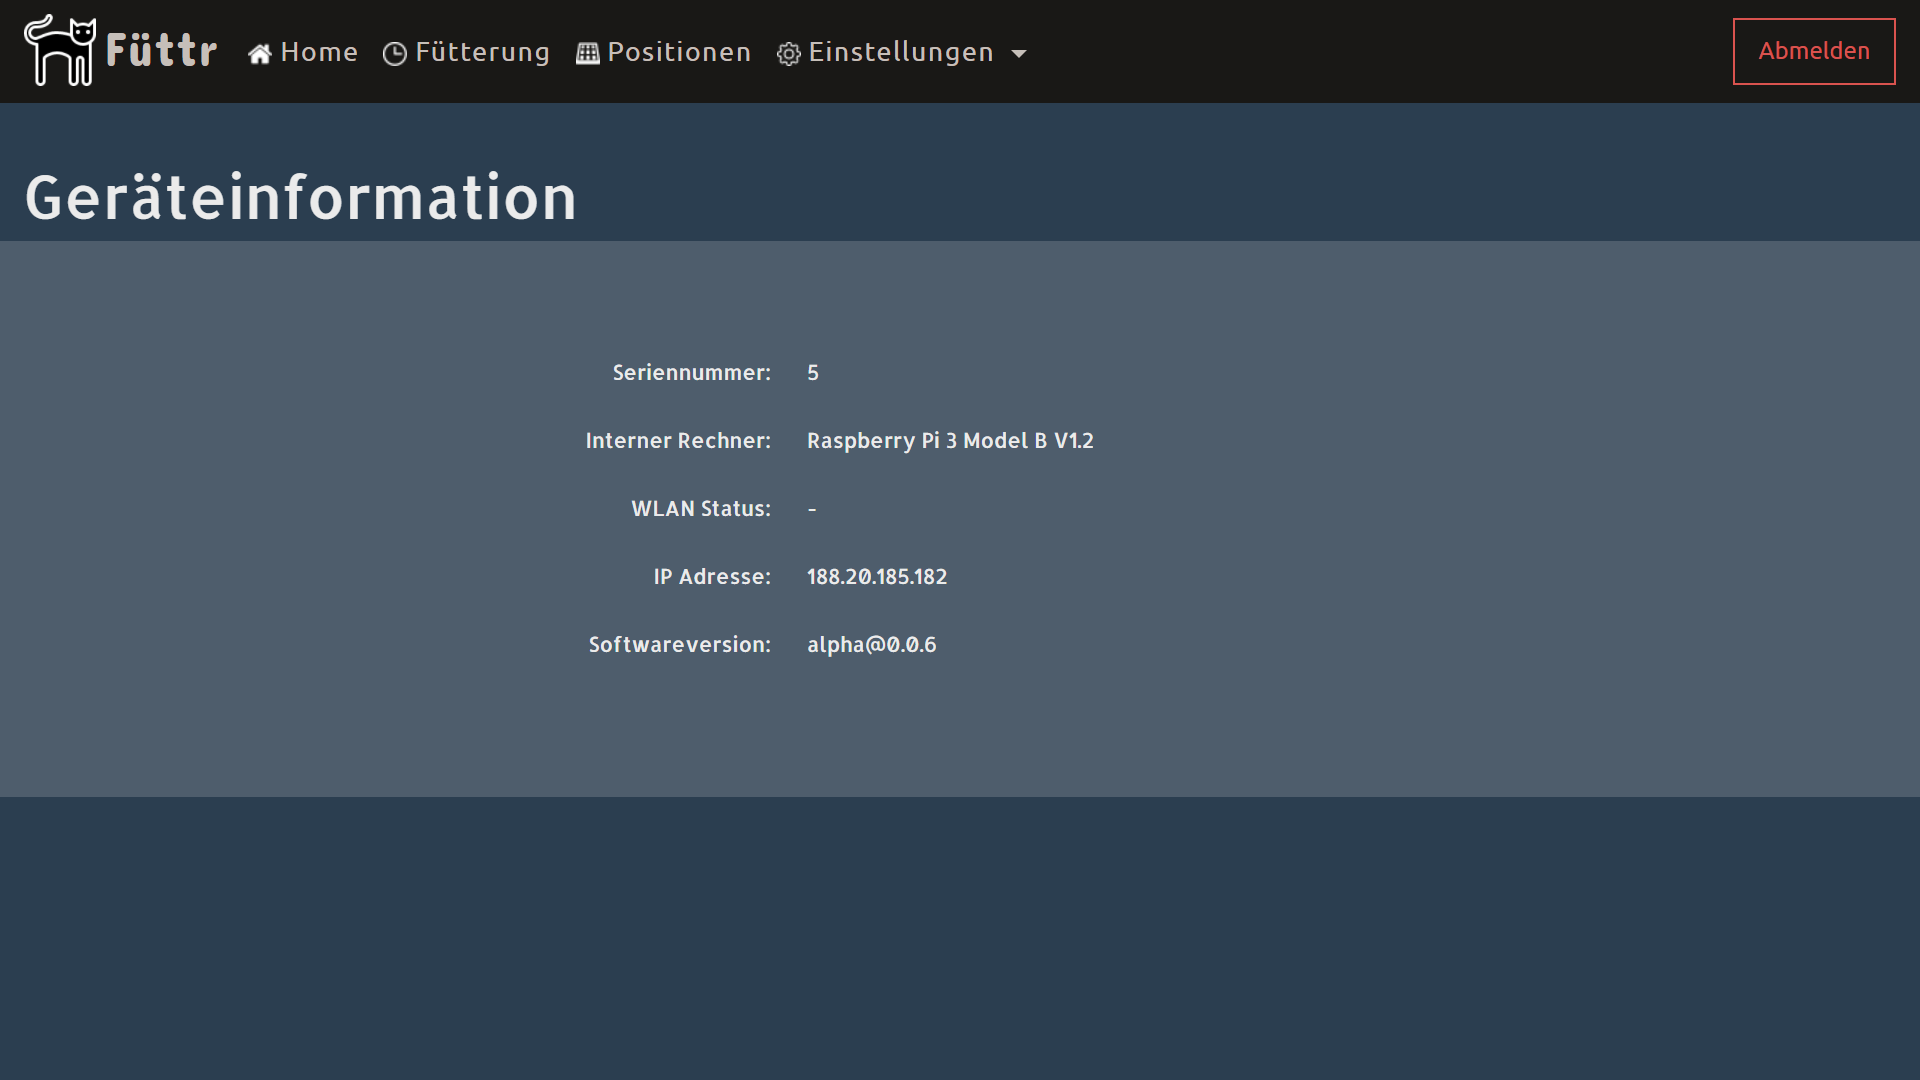
\includegraphics[width=0.7\textwidth]{Bilder/Greistorfer/Gerateinformation}
  \end{center}
  \caption{Geräteinformationen}
  \label{Geräteinformationen}
  \vspace{-50pt}
\end{wrapfigure}

Auf der Geräteinformations-Seite werden die wichtigsten Daten über das Gerät angezeigt. diese Daten sind:
\begin{itemize}
\item[•]Seriennummer
\item[•]Interner Rechner
\item[•]WLAN Status
\item[•]IP Adresse
\item[•]Softwareversion
\end{itemize}
Die Seriennummer ist eindeutig und wird von einem Server zugeteilt. Die IP-Adresse ist die aktuelle \textbf{externe} IP-Adresse. \\

\begin{wrapfigure}{r}{0.7\textwidth}
\vspace{-30pt}
  \begin{center}
    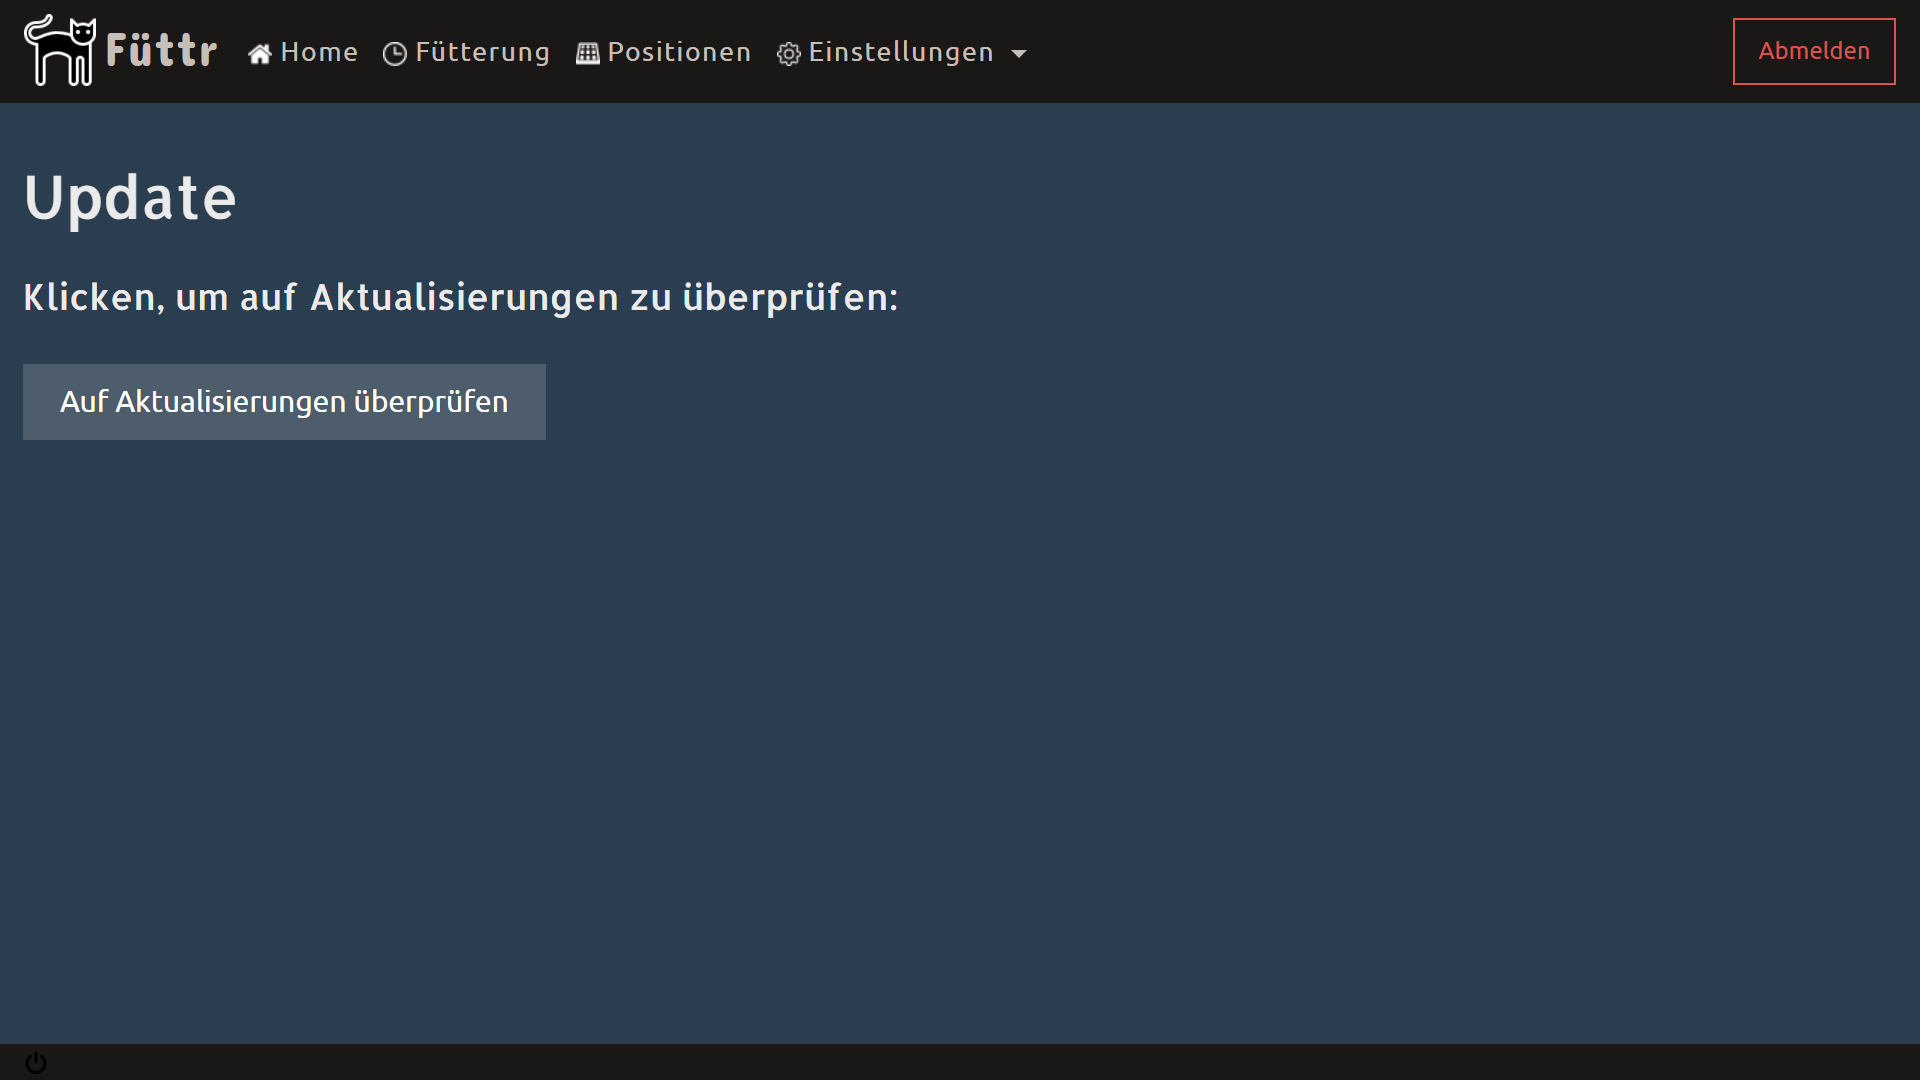
\includegraphics[width=0.7\textwidth]{Bilder/Greistorfer/Update}
  \end{center}
  \caption{Update}
  \label{Update}
  \vspace{-10pt}
\end{wrapfigure}

Auf der Update-Seite kann der Benutzer nach Updates suchen, Updates starten oder die Maschine herunterfahren. Wenn der Benutzer auf den Herunterfahren-Button klickt, der sich auf der linken Seite ganz unten befindet, wird er gewarnt, dass die Maschine nur mehr über das Aus- und wieder Einstecken des Netzteils startbar ist.\\

\subsubsection{Funktion}

\subsection{Server}

\subsubsection{Funktion}

\subsubsection{Mongodb}

\subsubsection{Kommunikation mit dem Java Programm}

\section{Zusammenfassung und Verbesserungsmöglichkeiten}
\renewcommand\appendixname{Anhang}
\renewcommand\appendixpagename{Anhang}
\renewcommand\appendixtocname{Anhang}

\lohead{}

\appendix
\begingroup
\makeatletter
\let\ps@plain\ps@empty
\appendixpage
\makeatother
\endgroup

\listoffigures
\listoftables
\lstlistoflistings
\chapter{Abkürzungsverzeichnis}
\begin{acronym}
	%Abkürzung hinzufügen: \acro{Kürzel}{Ausgeschrieben}
	\acro{npm}{Node Package Manager}
	\acro{JSON}{JavaScript Object Notation}
	\acro{JWT}{\ac{JSON} Web Token}
	\acro{DBS}{Database management System}
	\acro{API}{Application Programming Interface}
	\acro{HTML}{HyperText Markup Language}
\end{acronym}
%\bibliographystyle{jurabib}
\bibliographystyle{unsrt}
\bibliography{Literaturverzeichnis}

\end{document}